\subsection{(7Z)-13 ammoniotridec-7-enoate}

The first test case presented is relative to (7Z)-13 ammoniotridec-7-enoate, an
aminoacid zwitterion specifically designed to test the response of the
method to charge interactions (see Fig. \ref{fig:7Z-molecule}). The rigid
rotational behavior around the central double bond has been evaluated,
describing the absolute CAS+Single excitations (CAS+S) energy curves without
geometry relaxation with respect to the torsional dihedral angle. 

\begin{figure}[ht]
\begin{center}

\includegraphics[width=7cm,keepaspectratio]{02_localization/images/7Z-molecule.eps}
\caption{\footnotesize The (7Z)-13 ammoniotridec-7-enoate molecule. The cis-trans rigid
interconversion around the central double bond has been performed to test
the presented method. }
\label{fig:7Z-molecule}
\end{center}
\end{figure}



All the calculations have been performed by using ANO basis sets.
A minimal basis set ANO-1\cite{tca-77-291-1990} with
$2s1p$ contraction for C,N,O and $1s$ contraction for hydrogen atoms was
used.  The interatomic distances (in $\mbox{{\AA}ngstrom}$) are
r(C-C)=1.450, r(C=C)=1.335, r(C-H)=1.089, r(C-N)=1.440, r(N-H)=1.008,
r(C-O)=1.400. The angles are 109.5 degrees except for the C=C group and the
COO$^{-}$ group, where angles of 120 degrees have been used.
The dihedral angles were adjusted to obtain the cis and trans molecular
skeleton lying completely on the plane.

The CAS space selection consists of 2 electrons in 2 orbitals (C-C $\pi$
and $\pi^{*}$). This selection has been chosen to keep into account the
main correlative effects due to the rotation around the central
carbon-carbon double bond.

It must be stressed that, due to geometrical proximity, the interaction
between the charged groups affects the rotational behavior, and its
contribution must be kept into account.  For this reason, the two terminal groups
cannot be simply removed and replaced by hydrogen atoms.
As a comparison example, Fig.~\ref{fig:7Z-nocharges} shows the
behavior obtained by removing these groups and replacing them with
hydrogens. 

\begin{figure}[t]
\begin{center}
\includegraphics[width=8cm,angle=270]{02_localization/images/7Z-nocharges.eps}
\caption{\footnotesize A comparison of the CAS+S energy curves between the zwitterionic
(7Z)-13 ammoniotridec-7-enoate (solid line) and the (6Z)-dodec-6-ene, a
molecule obtained by replacing the charged NH$_{3}$ and COO$^{-}$ groups
with hydrogen atoms, dashed line.  A common zero in the energy scale of the
plot has been obtained taking the trans form as zero of the energy.  }
\label{fig:7Z-nocharges}
\end{center}
\end{figure}


Using the Freeze-and-Cut technique, the evaluation performed on a
small system reproduces the expected behavior: the freezing preserves the
electronic contribution of the groups, and the cut allows to work with a
reduced molecular system.

\begin{figure}[h!]
\begin{center}
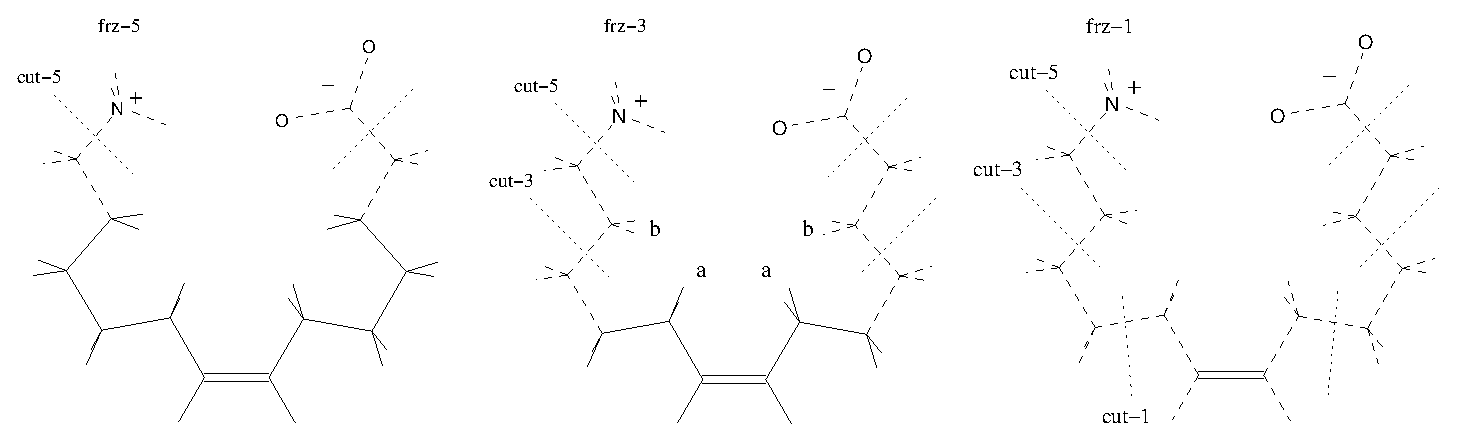
\includegraphics[width=12cm,keepaspectratio]{02_localization/images/7Z-frzcut-schema.eps}
\caption{\footnotesize (7Z)-13 ammoniotridec-7-enoate. Localized orbitals expressed on
atoms of the dashed line framework are frozen. Orbitals expressed on atoms
of the solid line framework are not frozen. Dotted lines depict the
cut seam. The cut is always performed on both chains, from ``cut-5'' (only
the charged groups are removed from the molecule, both left and right) to
``cut-1'' (maximal cut selection, only the central double bond and left and
right -CH$_{2}$- spacers are preserved). The ``a'' and ``b'' symbols in frz-3 picture
are labels for interesting hydrogen atoms. See text for details.  }
\label{fig:7Z-frzcut-schema}
\end{center}
\end{figure}


Different freeze and cut strategies have been chosen in order to evaluate
the behavior of our technique with respect to these selections.
Three freezing levels, labeled ``frz-1,'' ``frz-3'' and ``frz-5'' have been
defined (Fig. \ref{fig:7Z-frzcut-schema}), and also a ``nofrz'' level
where no freezing has been performed.  The $1s$ core atomic orbitals for heavy
atoms have been frozen at SCF level regardless of the atom positions.

The cut strategy follows the freezing strategy. Four cut thresholds have
been chosen, with labels ``cut-1,'' ``cut-3,'' ``cut-5'' and ``nocut,''
following the freezing choice, but preserving a -CH$_2$-
spacer between the last not frozen orbital and the first cutout atom.

The analysis performed at 0 (cis) and 180 (trans) degrees and their
difference are presented in Tab. \ref{tbl:7Z-cis-trans-diff}

\begin{center}
\begin{threeparttable}
\begin{tabular}{lcccc}
\hline
    		&		nofrz			&	frz-5				&	frz-3				&	frz-1	\\	
\hline
			&	\multicolumn{4}{c}{Cis} \\
nocut		&	-709.483006     	&	-709.482889     	&	-709.482281     	&	-709.465687      \\
cut-5		&						&	-709.373507  		&   -709.479395  		&	-709.465638      \\
cut-3		&						&						&	-709.218388     	&	-709.460918      \\
cut-1		&						&						&						&	-709.357068    	 \\
			&	\multicolumn{4}{c}{Trans} \\
nocut		&	-709.388878     	&	-709.388760     	&	-709.388156     	&	-709.371500      \\
cut-5		&						&	-709.279814  		&   -709.385430  		&	-709.371437      \\
cut-3		&						&						&	-709.123318     	&	-709.366578      \\
cut-1		&						&						&						&	-709.258750    	 \\
			&	\multicolumn{4}{c}{Diff} \\
nocut		&	59.0267         	&	59.0272         	&	59.0251         	&	59.0640        	 \\
cut-5		&						&	58.7538         	&	58.9248         	&	59.0725          \\
cut-3		&						&						&	59.6173         	&	59.1598          \\
cut-1		&						&						&						&	61.6542        	 \\
\hline
\end{tabular}
\caption{\footnotesize CAS+S absolute energies (Hartree) and energy
difference (kcal/mol) between (7Z)-13 ammoniotridec-7-enoate cis and trans
structure, with respect to different freeze and cut strategies.}
\label{tbl:7Z-cis-trans-diff}
\end{threeparttable}
\end{center}


It can be seen that the cut technique produces energy differences between
cis and trans that are comparable to the reference value obtained with no
cut and freeze.

A different behavior can be evaluated for the difference between the 0 degrees
form and the 90 degrees form (Tab. \ref{tbl:7Z-diff-cis-90})

\begin{center}
\begin{threeparttable}
\begin{tabular}{lcccc}
\hline
			&		nofrz			&	frz-5				&	frz-3				&	frz-1	\\
\hline
nocut		&	130.4145        	&	130.4953        	&	131.2643        	&	167.4817         \\
cut-5		&						&	130.1703        	&	131.1572        	&	167.5065         \\
cut-3		&						&						&	130.8074        	&	168.4879         \\
cut-1		&						&						&						&	171.2689       	\\
\hline
\end{tabular}
\caption{\footnotesize CAS+S energy difference (kcal/mol) between the (7Z)-13
ammoniotridec-7-enoate cis and the 90 degrees twisted structure with respect
to different freeze and cut strategies.}
\label{tbl:7Z-diff-cis-90}
\end{threeparttable}
\end{center}


The frz-1 selection presents a large deviation from the expected value. This
arises from the fact that the SCF at 90 degrees evaluates very poorly the
orbitals involved (directly or indirectly) in the bond breaking. 

This leads to an initial bad description of the orbitals, which are frozen
at this poor quality level. As a consequence, the optimization guess is
affected by this initial description. By relaxing the freeze selection,
these orbitals are allowed to improve in the subsequent iterative process,
thus drastically reducing the incorrect behavior. In the case of frz-1
strategy, however, the effects are too pronounced to be smoothed out.

\begin{figure}[h!]
\begin{center}
\includegraphics[width=8cm,keepaspectratio,angle=270]{02_localization/images/7Z-frz-1.eps}
\caption{\footnotesize CAS+S energy curves (Hartree) for the cis-trans rigid
interconversion of the (7Z)-13 ammoniotridec-7-enoate with different 
cut strategies and frz-1 freeze strategy. The reference (solid black line)
is evaluated on the complete molecular system with no frozen orbitals except
the $1s$ core orbital for heavy atoms. frz-1/nocut curve (dotted line,
$\Box$ symbol) and frz-1/cut-5 (short dash line, $\times$ symbol) appear as
superposed on the drawing scale. The other curves are frz-1/cut-3 (long
dash line, $\bigcirc$ symbol) and frz-1/cut-1 (dot-dash line, $\Diamond$
symbol).  }
\label{fig:7Z-frz-1}
\end{center}
\end{figure}



This is of particular evidence in the curve diagrams depicted in
Fig.~\ref{fig:7Z-frz-1}: the solid line is the nofrz/nocut reference,
obtained by interpolating points from 0 to 180 (step 10 degrees) with a
cubic spline curve. The other curves represent the incorrect behavior of
frz-1 with cut strategies cut-1, cut-3, cut-5 and nocut (these last two
curves are superposed).  Each point has been generated using as a starting
guess the converged orbitals from the previous point on the complete AO
space (the ORTORBL matrix at convergence). Depending on the guess (70 or 110
degrees), two different curves can be obtained, giving a spike at 90
degrees.  This reflects the dependence on the SCF solution, which affects
the frozen orbital framework. It is however important to note that these
curves are still parallel to the reference curve when far from the 90
degrees region. 

As can be seen from Fig. \ref{fig:7Z-frz-3}, this incorrect behavior is
drastically reduced by going from frz-1 to frz-3.

\begin{figure}[ht]
\begin{center}
\includegraphics[width=8cm,angle=270]{02_localization/images/7Z-frz-3.eps}
\caption{\footnotesize CAS+S energy curves (Hartree) for the cis-trans rigid
interconversion of the (7Z)-13 ammoniotridec-7-enoate with different 
cut strategies and frz-3 freeze strategy. The reference (solid black line,
see caption of Fig.\ref{fig:7Z-frz-1} for details),
frz-3/nocut curve (dotted line, $\Box$ symbol) and frz-3/cut-5 (short
dash line, $\times$ symbol) appear nearly superposed on the drawing
scale. The other curve is frz-3/cut-3 (long dash line, $\bigcirc$ symbol).
}
\label{fig:7Z-frz-3}
\end{center}
\end{figure}


The curves are nearly parallel to the reference, but with a strong energy
shift between cut-3 and cut-5.
This difference is principally due to the four non-frozen C-H bonds (marked
with the ``a'' labels in Fig. \ref{fig:7Z-frzcut-schema}): they are
described by hydrogen atoms (marked with the ``b'' labels)
that have been cut out from the small system in the cut-3 analysis. This
results in a shift in absolute energies, but does not affect the relative
behavior.

Treating the same cut-3 system, but also adding the ``b'' hydrogen atoms
gives CAS+S energies in better accord with the frz-3/cut-5 values,
providing nearly half of the gap between frz-3/cut-3 and frz-3/cut-5.
%(see Tab. \ref{tbl:7Z-trend}).
\begin{center}
\begin{threeparttable}
\begin{tabular*}{0.80\textwidth}{l@{\hspace*{10mm}}cccc}
\hline
					&	cis			&	trans			&	diff   \\
\hline
frz-3/cut-5			&	-709.479395      	&	-709.385430        	&  58.9248 \\
frz-3/cut-3+H$_{\mbox{b}}$	&	-709.374870			&	-709.280646       	&  59.0873 \\
frz-3/cut-3			&	-709.218388			&	-709.123318			&  59.6173 \\
\hline
\end{tabular*}
\caption{\footnotesize CAS+S absolute energies (Hartree) and energy
difference (kcal/mol) between (7Z)-13 ammoniotridec-7-enoate cis and trans
for frz-3/cut-3, frz-3/cut-5 and the intermediate frz-3/cut-3+H$_b$, where
hydrogens labeled ``b'' in Fig.  \ref{fig:7Z-frzcut-schema}
have been preserved for the cut-3 strategy.}
\label{tbl:7Z-trend}
\end{threeparttable}
\end{center}

This confirms the importance of these four hydrogens for the evaluation
of the absolute energy, but the relative behavior is unaffected.
The same effect arises in all the diagonal values of the absolute energy
tables, where a similar situation happens due to the proximity of
the cut seam to the non-frozen orbitals.

The frz-3 selection has also been studied with a larger CAS space.
This has been obtained by enriching the previous space with the C-C $\sigma$
and $\sigma^{*}$ orbitals, thus leading to a 4 electron in 4 orbitals space.
\begin{figure}[h!]
\begin{center}
\includegraphics[width=78mm,angle=270]{02_localization/images/7Z-frz-3-cas44.eps}
\caption{\footnotesize CAS+S energy curves (Hartree) for the cis-trans rigid
interconversion of the (7Z)-13 ammoniotridec-7-enoate with an extended CAS
defined as 4 electrons in 4 orbitals, with different cut strategies for the
frz-3 freeze strategy. The reference (solid black line, see caption of
Fig.\ref{fig:7Z-frz-1} for details), frz-3/nocut curve (dotted line,
$\Box$ symbol) and frz-3/cut-5 (short dash line, $\times$ symbol) appear
nearly superposed on the drawing scale. The other curve is frz-3/cut-3 (long
dash line, $\bigcirc$ symbol).
}
\label{fig:7Z-frz-3-cas44}
\end{center}
\end{figure}


The evaluation has been performed at 90 degrees and from 0 to 180 degrees
with a step of 20 degrees, interpolating the points with a cubic spline curve.

As can be seen from Fig. \ref{fig:7Z-frz-3-cas44} the same correct
behavior is obtained, the only difference being the shift of the energy due
to the larger CAS space. The relative energy for the frz-3/cut-3 is, for
example, 59.6149 kcal/mol. This value is in a very good accord with the one
obtained using the CAS 2/2 space, 59.6173 kcal/mol.

Fig. \ref{fig:7Z-frz-5} finally depicts the results for frz-5 strategy with the
CAS 2/2 space, where frz-5/cut-5 curve lays higher in energy but still
parallel to the reference curve, and the frz-5/nocut curve nearly superposed
to the reference. 
\begin{figure}[ht]
\begin{center}
\includegraphics[width=8cm,angle=270]{02_localization/images/7Z-frz-5.eps}
\caption{\footnotesize CAS+S energy curves (Hartree) for the cis-trans rigid
interconversion of the (7Z)-13 ammoniotridec-7-enoate with different cut
strategies and frz-5 freeze strategy. The reference (solid black line, see
caption of Fig.\ref{fig:7Z-frz-1} for details) and frz-5/nocut curve
(dotted line, $\Box$ symbol) appear as superposed on the drawing scale.  The
other curve is frz-5/cut-5 (short dash line, $\times$ symbol) 
}
\label{fig:7Z-frz-5}
\end{center}
\end{figure}


Fig.\ref{fig:7Z-orbitals} shows the optimized $\pi$ orbital for the cis
molecule with different cut strategies at frz-1 level of freeze. The plots
have been realized with the Molden program\cite{molden-site} with a contour
factor of 0.002. We can note that the cut-5 strategy does not change the
orbital in a significant way, due to the graphically negligible expression
of the orthogonalization tail of the orbital on the removed fragments.  The
cut-3 and cut-1 strategies show instead the confinement of the optimized
orbital inside the group of atoms on which the projection was performed.
The small lobes for the $\pi$ description are removed by the cut procedure,
and the optimization preserves the locality imposed by the method.

%\begin{wrapfigure}{l}{65mm}
%\vspace{3mm}
%\end{wrapfigure}
\begin{center}
\begin{figure}[h!]
\begin{center}
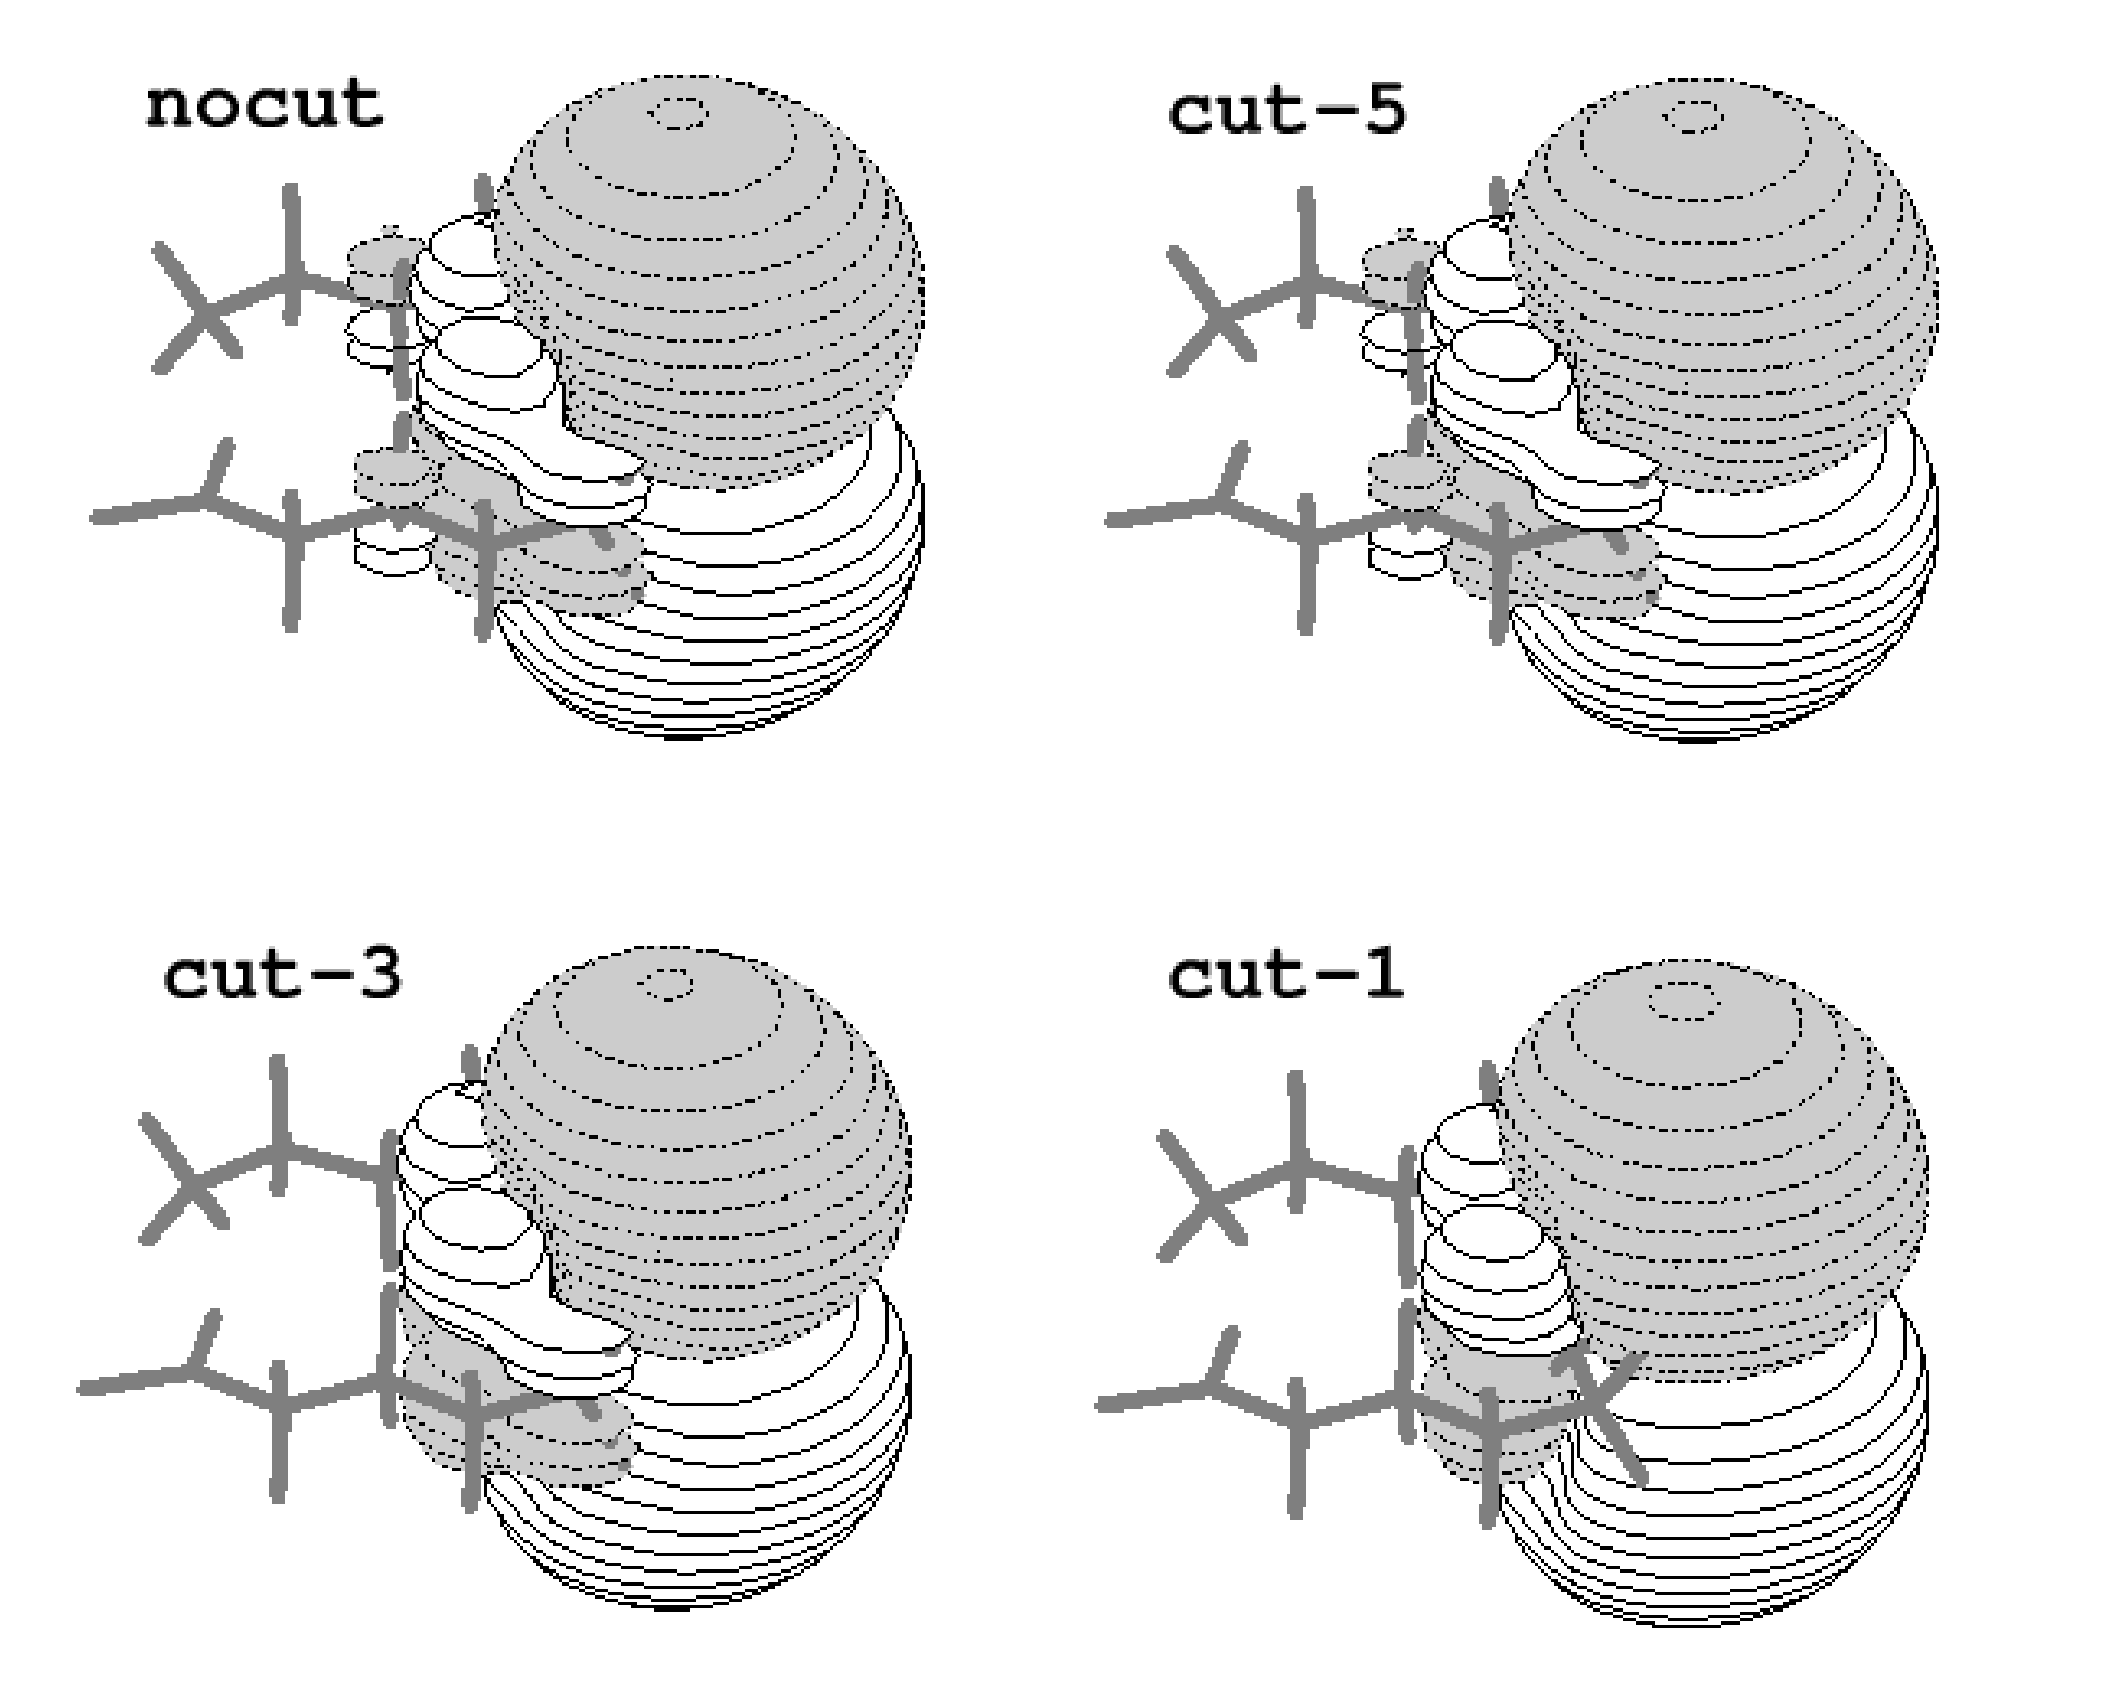
\includegraphics[width=72mm,keepaspectratio]{02_localization/images/7Z-orbitals.eps}
\caption{\footnotesize The $\pi$ orbital representation with respect to different cut strategies at frz-1
freeze strategy. }
\label{fig:7Z-orbitals}
\end{center}
\end{figure}
\end{center}



The improvements in timings are presented as an example in Tab. \ref{tbl:timings},
applied to the (7Z)-13 ammoniotridec-7-enoate with the CAS 2/2 space.

As can be seen, performing the integral evaluation on the reduced
system is a lightweight process.
Nocut evaluations have a value of zero for the reduced system. The integral
evaluation on the complete system can be used in this case, saving the cost
of a new evaluation.

The remaining steps are quite fast, but the best compromise between result
quality and time is for the frz-3/cut-3 evaluation.
In this case a reduction of the time needed to perform the optimization is
counterbalanced by the need of an integral evaluation on the small system,
but the difference between the frz-3/cut-3 and the frz-3/nocut becomes
dramatic when working on systems larger than the presented ones, which are
the final targets of this technique.

\begin{center}
\begin{table}[ht]
\footnotesize
\begin{center}
\begin{tabular}{lcccccc}
\hline
				&	seward-large	&	seward-small		&	large	& small	&	CAS+S	&	total \\
\hline
nofrz/nocut		&	1009			&			0			&	50		&	39		&	1062	&	2160 \\
frz-5/nocut		&	1009			&			0			&	50		&	19		&	355		&	1433 \\
frz-5/cut-5		&	1009			&			433			&	50		&	6		&	225		&	1723 \\
frz-3/nocut		&	1009			&			0			&	50		&	7		&	184		&	1250 \\
frz-3/cut-3		&	1009			&			100			&	50		&	1		&	99		&	1259 \\
frz-1/nocut		&	1009			&			0			&	50		&	2		&	43		&	1104 \\
frz-1/cut-1		&	1009			&			8			&	50		&	0		&	18		&	1085 \\
\hline
\end{tabular}
\end{center}
\caption{\footnotesize Timings (in seconds) for evaluations performed on (7Z)-13
ammoniotridec-7-enoate, against different freeze and cut strategies. Test
performed on Intel dual Xeon 2.8 GHz 2 GB RAM. ``seward-large'' and ``seward-small''
are the timings for the AO integral evaluation. ``large'' and ``small'' columns
represents the timings needed for the creation of the transformed integrals
which will seed the first iteration. ``CAS+S'' column reports the timings for
the complete iterative procedure up to the convergence.}
\label{tbl:timings}
\end{table}
\end{center}


